\begin{exercise}\label{ex:020302}
    Construct a syntax directed translation scheme that translates arithmetic 
    expressions from postfix notation into infix notation. Give annotated parse 
    trees for the inputs \texttt{95-2*} and \texttt{952*-}.
\end{exercise}
\begin{solution}\label{sol:020302}
    The translation scheme is given below.
    \begin{align*}
        E \yld\ &E\ \cbrak{\text{print(`\texttt{+}')}}\ E\ \texttt{+} \\
             |\ &E\ \cbrak{\text{print(`\texttt{-}')}}\ E\ \texttt{-} \\
             |\ &E\ \cbrak{\text{print(`\texttt{*}')}}\ E\ \texttt{*} \\
             |\ &E\ \cbrak{\text{print(`\texttt{/}')}}\ E\ \texttt{/} \\
             |\ &\cbrak{\text{print(`\texttt{num}')}}\ num
    \end{align*}
    The parse trees for the inputs \texttt{95-2*} and \texttt{952*-} are shown 
    in \autoref{fig:020302a} and \autoref{fig:020302b}.
    \begin{figure}[!ht]
    \centering
    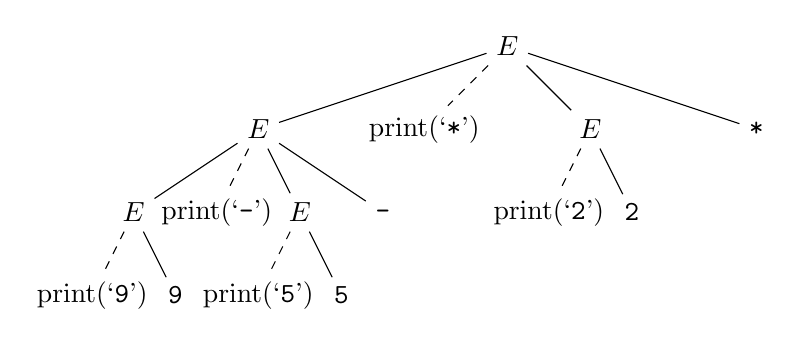
\begin{tikzpicture}
        [
            level distance = 3em, 
            level 1/.style={sibling distance=6em},
            level 2/.style={sibling distance=3em},
        ]
        \node {$E$}
        child {
            node {$E$}
            child {
                node {$E$}
                child {
                    node {print(`\texttt{9}')} edge from parent[dashed]
                }
                child {node {\texttt{9}}}
            }
            child {
                node {print(`\texttt{-}')} edge from parent[dashed]
            }
            child {
                node {$E$}
                child {
                    node {print(`\texttt{5}')} edge from parent[dashed]
                }
                child {node {\texttt{5}}}
            }
            child {node {\texttt{-}}}
        }
        child {
            node {print(`\texttt{*}')} edge from parent[dashed]
        }
        child {
            node {$E$}
            child {node {print(`\texttt{2}')} edge from parent[dashed]}
            child {node {\texttt{2}}}
        }
        child {node {\texttt{*}}}
        ;
    \end{tikzpicture}
    \caption{Parse tree for the input \texttt{95-2*} for \cref{ex:020302}.}
    \label{fig:020302a}
\end{figure}

    \begin{figure}[!ht]
    \centering
    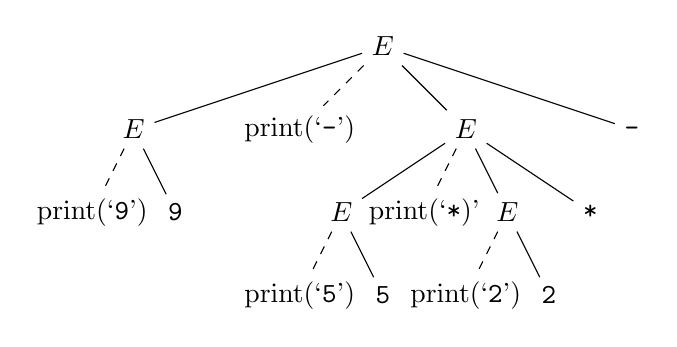
\begin{tikzpicture}
        [
            level distance = 3em, 
            level 1/.style={sibling distance=6em},
            level 2/.style={sibling distance=3em},
        ]
        \node {$E$}
        child {
            node {$E$}
            child {node {print(`\texttt{9}')} edge from parent[dashed]}
            child {node {\texttt{9}}}
        }
        child {node {print(`\texttt{-}')} edge from parent[dashed]}
        child {
            node {$E$}
            child {
                node {$E$}
                child {node {print(`\texttt{5}')} edge from parent[dashed]}
                child {node {\texttt{5}}}
            }
            child {node {print(`\texttt{*})'} edge from parent[dashed]}
            child {
                node {$E$}
                child {node {print(`\texttt{2}')} edge from parent[dashed]}
                child {node {\texttt{2}}}
            }
            child {node {\texttt{*}}}
        }
        child {node {\texttt{-}}}
        ;
    \end{tikzpicture}
    \caption{Parse tree for the input \texttt{952*-} for \cref{ex:020302}.}
    \label{fig:020302b}
\end{figure}
\end{solution}